\section{Test n°1}

\begin{description}
 \item[Date]: 18/05/15
 \item[Sur code révisé]: commit f7da39f0001d221ccd82f236781b4c97f7f9ca88
 \item[OS]: Linux Mint 17 Cinnamon 64-bit
 \item[Noyau Linux]: 3.31.0-24-generic
 \item[Processeur]: Intel© Core™ i5-3230M CPU @ 2.60GHz * 2
 \item[Type d'algorithme]: mono-thread
 \item[Objectif]: Prouvé l'utilité de l'algorithme de réduction des points de départ.
\end{description}

\begin{figure}[h]
\begin{tabular}{|*{5}{c|}}
\hline
Algorithme&Taille du cube&Temps de calcul (s)&Solutions&Chemins explorés \\
\hline
\multirow{3}{*}{Actif}&2x2x2&0,000429&6&38 \\
&3x3x3&0,047914&32&91 347 \\
&4x4x4&140,208572&11&615 765 110 \\
\hline
\multirow{3}{*}{Inactif}&2x2x2&0,005929&144&889 \\
&3x3x3&0,781355&576&1 922 269 \\
&4x4x4&2985,381852&192&11 258 895 649 \\
\hline
\end{tabular}
\caption{Résultats du test n°1}
\end{figure}

\newpage

\paragraph{Interprétation} La première interprétation que l'on peut faire de ses résultats, c'est que sans surprise, plus la taille du cube est grande, plus le temps de calcul est important (0,000429 secondes pour un 2x2x2 contre 140,208572 pour un 4x4x4). Ces résultat nous permettent également de prouver l'efficacité de notre algorithme de réduction des points de départ. En effet lorsque l'algorithme est actif on constate que les temps de calcul, tout comme le nombre de chemins explorés, sont plus faibles que lorsque qu'il est inactif.

\begin{figure}[h]
 \centering
 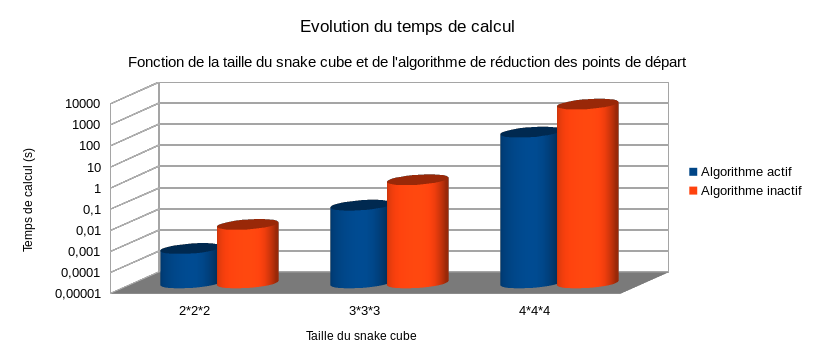
\includegraphics[scale=0.6,keepaspectratio=true]{img/test1.png}
 \caption{Graphique test n°1}
\end{figure}

\newpage

\section{Test n°2}

\begin{description}
 \item[Date]: 30/05/15
 \item[Sur code révisé]: commit c8d1b7bdf5eb1f94255cd66aca9b0b800cba838d
 \item[OS]: Linux Mint 17 Cinnamon 64-bit
 \item[Noyau Linux]: 3.31.0-24-generic
 \item[Processeur]: Intel© Core™ i5-3230M CPU @ 2.60GHz * 2
 \item[Type d'algorithme]: mono-thread ou multi-thread
 \item[Objectif]: Évaluer l'efficacité de la parallélisation du calcul des solutions.
\end{description}

\begin{figure}[h]
\begin{center}
\begin{tabular}{|*{2}{c|}}
\hline
\multicolumn{2}{|c|}{Snake 3x3x3} \\
\hline
Nombre de thread & Temps d’exécution (s) \\
\hline
1 & 0,002462 \\
\hline
2 & 0,001642 \\
\hline
3 & 0,003461 \\
\hline
4 & 0,002232 \\
\hline
5 & 0,002773 \\
\hline
6 & 0,002652 \\
\hline
7 & 0,002292 \\
\hline
8 & 0,001988 \\
\hline
9 & 0,002477 \\
\hline
10 & 0,002387 \\
\hline
\end{tabular}
\end{center}
\caption{Résultats du test n°2-1}
\end{figure}

\begin{figure}[h]
\begin{center}
\begin{tabular}{|*{2}{c|}}
\hline
\multicolumn{2}{|c|}{Snake 4x4x4} \\
\hline
Nombre de thread & Temps d’exécution (s) \\
\hline
1 & 99,067031 \\
\hline
2 & 67,078735 \\
\hline
3 & 65,022525 \\
\hline
4 & 53,198234 \\
\hline
5 & 47,776286 \\
\hline
6 & 71,80401 \\
\hline
7 & 54,967149 \\
\hline
8 & 47,836183 \\
\hline
9 & 45,215047 \\
\hline
10 & 45,38195 \\
\hline
\end{tabular}
\end{center}
\caption{Résultats du test n°2-2}
\end{figure}

\newpage

\paragraph{Interprétation} Le temps de résolution du snake 3x3x3 étant très cours, l'efficacité du calcul parallèle est difficile à percevoir. De plus, l'influence des autres processus lancés sur la machine dans l’ordonnancement et donc dans le sur le temps (réel) d'exécution du calcul n'est pas négligeable dans le cas du 3x3x3. Le cas du snake 4x4x4 est plus intéressant. On constate que plus on affecte de thread à la résolution du calcul, moins celui-ci prend de temps jusqu'à ce que l'on arrive à 6 thread. A ce moment là, on observe un ``pic'' dans le temps de calcul puis il décroit de nouveau. Selon nous, la raison de ce pic est dû à la façon dont nous avons implémenté le système de répartition des points de départ à traiter pour chaque thread. Dans ce cas précis, il y a 10 points de départ à traiter. Si l'on utilise 6 thread de calcul, le programme affecte (10 / 6) = 1 point de départ pour chaque thread, excepté le dernier auquel il affecte (10 - 5) = 5 thread. Finalement, avec ce système, on constate que la parallélisation du calcul n'est vraiment pas optimale, ce qui explique le ``pic '' dans le graphe.

\begin{figure}[h]
 \centering
 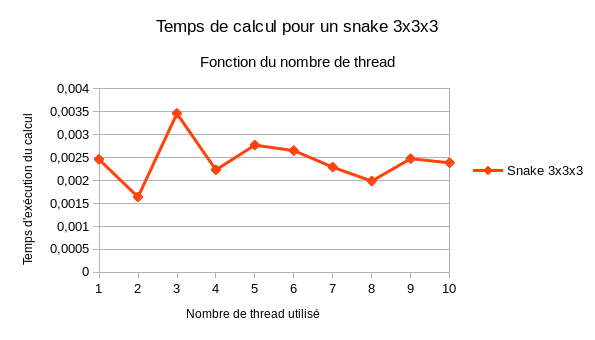
\includegraphics[scale=0.7,keepaspectratio=true]{img/test2-1.png}
 \caption{Graphique test n°2-1}
\end{figure}

\begin{figure}[h]
 \centering
 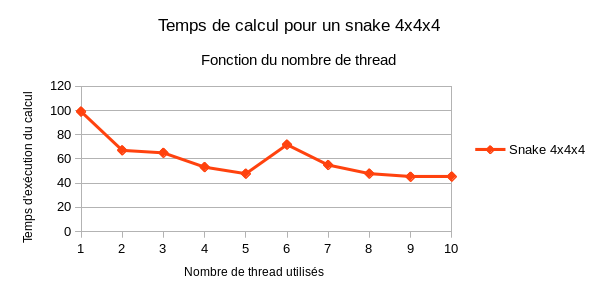
\includegraphics[scale=0.7,keepaspectratio=true]{img/test2-2.png}
 \caption{Graphique test n°2-2}
\end{figure}

\section{Limites}